\documentclass{beamer}

\usepackage[utf8]{inputenc}
\usepackage{graphicx}
\graphicspath{ {./images/} }
\usepackage{subcaption}

\usepackage{enumitem}
\setlist{itemsep=10pt}
\setitemize{label=\usebeamerfont*{itemize item}%
  \usebeamercolor[fg]{itemize item}
  \usebeamertemplate{itemize item}}

%Information to be included in the title page:
\title{Abelian Sandpile Basics}
%\author{Anonymous}
%\institute{ShareLaTeX}
\date{2018}



\begin{document}

\frame{\titlepage}

\begin{frame}
\frametitle{Abelian Sandpile Model}
\begin{itemize}
\item Rough model of a pile of sand, based on a finite directed (multi-) graph $G$, with vertices $V$ and edges $E$.

\item Chips (grains of sand) are stacked on the vertices.

\item Chips can flow to other vertices via edges of $G$.

\item Originally studied on uniform grids.

\item Also known as the chip-firing game.
\end{itemize}
\end{frame}

\begin{frame}
\frametitle{Chip-Firing}
\begin{itemize}
\item Let $n_i$ be the number of chips on vertex $v_i$
\item Let $e_{i} = \{e \in E : e \mbox{ starts at } v_i\}$

\item If a vertex $n_i \geq |e_{v_i}|$ it can \textbf{fire}.

\item When a vertex fires, it transfers a chip down each of its \textbf{outbound} edges.
\end{itemize}


\end{frame}

\begin{frame}
\frametitle{}

%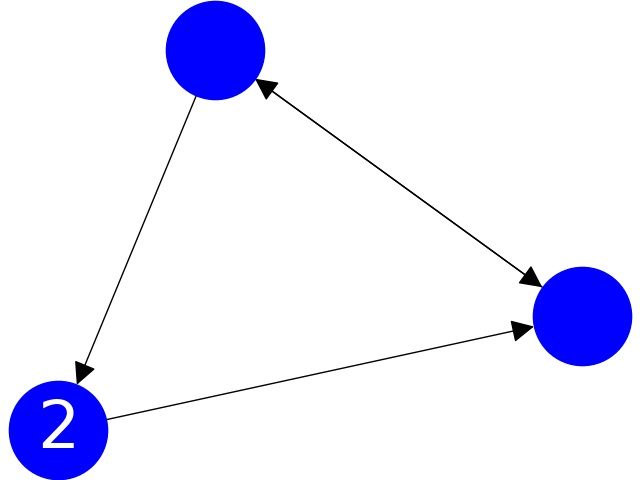
\includegraphics[width=0.5\textwidth]{sandpile_simple_0}%
%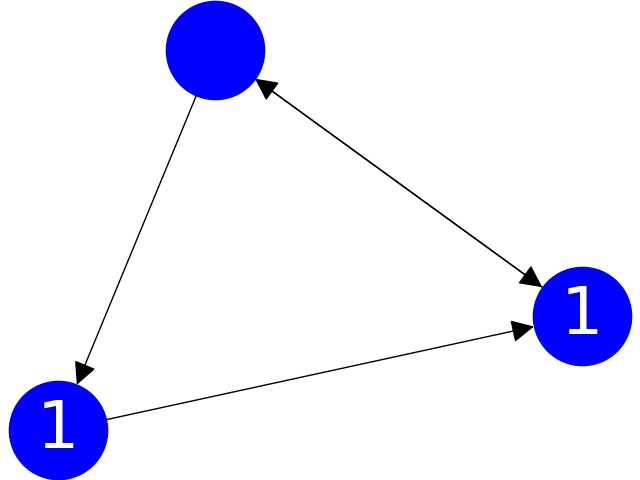
\includegraphics[width=0.5\textwidth]{sandpile_simple_1}

\begin{figure}[h!]
  \centering
  \begin{subfigure}[b]{0.4\linewidth}
    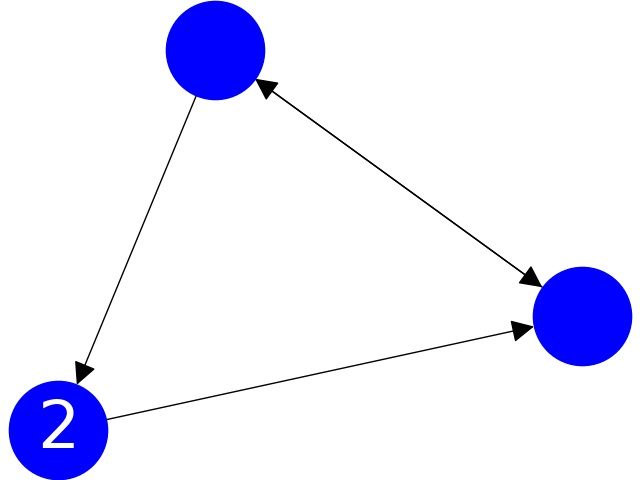
\includegraphics[width=\linewidth]{sandpile_simple_0}
    \caption{Before firing: Lower left vertex has one outbound edge and two chips.}
  \end{subfigure}
  \begin{subfigure}[b]{0.4\linewidth}
    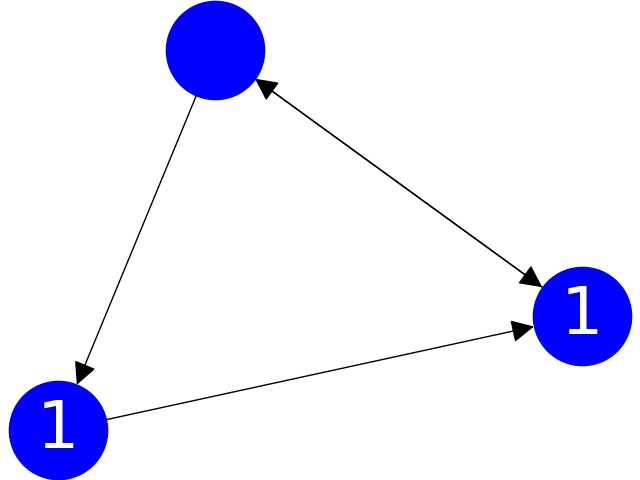
\includegraphics[width=\linewidth]{sandpile_simple_1}
    \caption{After firing: One chip has been transferred to the far right vertex.}
  \end{subfigure}
  \caption{Firing example.}
  \label{fig:coffee}
\end{figure}

\end{frame}


\begin{frame}
\frametitle{Chip Configuration}

%If $n_i$ is the number of chips on vertex $v_i$, the chip \textbf{configuration}
%is the set of pairs $\{(v_i,n_i) : v_i \in V\}$.

%If we fix an ordering of $V$,
\end{frame}

\begin{frame}
\frametitle{Stable Configuration}

\end{frame}


\begin{frame}
\frametitle{``Sink''}

%A vertex $v$ of $G$ with no outbound edges is known as a ``sink''.



\end{frame}

\begin{frame}
\frametitle{Reduced Laplacian}

\end{frame}

\begin{frame}
\frametitle{Chip Configuration Revisited}

\end{frame}

\begin{frame}
\frametitle{Stabilizing}

\end{frame}


\begin{frame}
\frametitle{Firing ``History''}

\end{frame}

\begin{frame}
\frametitle{Chip Addition Operator}

\end{frame}


\end{document}





\begin{frame}
\frametitle{}

\end{frame}
